\documentclass{article}
\usepackage[utf8]{inputenc}
\usepackage[a4paper, margin=1in]{geometry}
\usepackage{siunitx}
\usepackage{amsmath}
\usepackage{enumitem}
\usepackage{esdiff}
\usepackage{pgfplots}

\pgfplotsset{compat=1.18, width=10cm}

\tolerance=1
\emergencystretch=\maxdimen
\hyphenpenalty=10000
\hbadness=10000

\sisetup{
    input-ignore={.},
    output-decimal-marker={,},
    group-minimum-digits=4,
    group-separator={.},
    group-digits=integer
}

\newcommand{\penyelesaian}{\textbf{Penyelesaian: }}

\title{\textbf{Komputasi Numerik: Tugas 2}}
\author{Kelompok 15}
\date{}

\begin{document}

\maketitle

\begin{enumerate}
    \item Dengan metode grafik, dapatkan akar-akar persamaan:
    \begin{enumerate}
        \item $e^x - x - 2 = 0$ \\
        \penyelesaian $e^x - x - 2 = 0 \Leftrightarrow e^x = x + 2$, sehingga diperoleh dua persamaan $y = e^x$ dan $y = x + 2$. 
        Grafik dari kedua persamaan tersebut diperoleh sebagai berikut.
        \begin{center}
            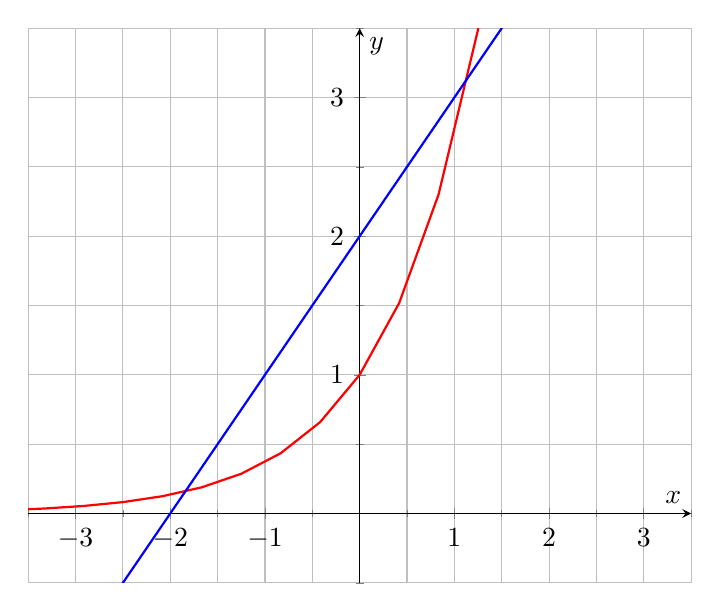
\begin{tikzpicture}
                \begin{axis}[grid=both,ymin=-0.5,ymax=3.5,xmax=3.5,xmin=-3.5,
                             minor tick num=1,axis lines = middle,xlabel=$x$,ylabel=$y$]
                    \addplot[color=red, thick]{e^x};
                    \addplot[color=blue, thick]{x+2};
                \end{axis}
            \end{tikzpicture}
        \end{center}
        Berdasarkan letak perpotongan garis dari dua persamaan, diperoleh dua akar, yakni $x_1$ yang terletak di antara $(-2, 1)$ dan $x_2$ yang terletak di antara $(1, 2)$.

        \item $10^x = 100 - 2x$ \\
        \penyelesaian Diperoleh dua persamaan, $y = 10^x$ dan $y = 100 - 2x$. Berikut hasil plot dari kedua persamaan tersebut.
        \begin{center}
            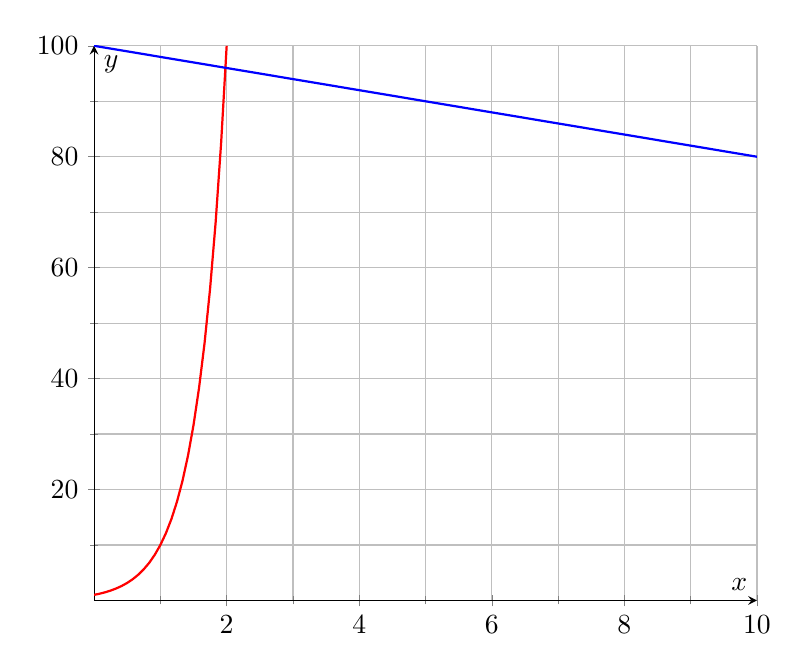
\begin{tikzpicture}
                \begin{axis}[grid=both,ymin=0,ymax=100,xmax=10,xmin=0,
                             minor tick num=1,axis lines = middle,xlabel=$x$,ylabel=$y$]
                    \addplot[red, thick, domain=0:2]{10^x};
                    \addplot[color=blue, thick, domain=0:10]{100-2*x};
                \end{axis}
            \end{tikzpicture}
        \end{center}
        Berdasarkan letak perpotongan dua garis, diperoleh informasi bahwa fungsi hanya memiliki satu akar $x$.

        Grafik diperbesar pada akar $x$:
        \begin{center}
            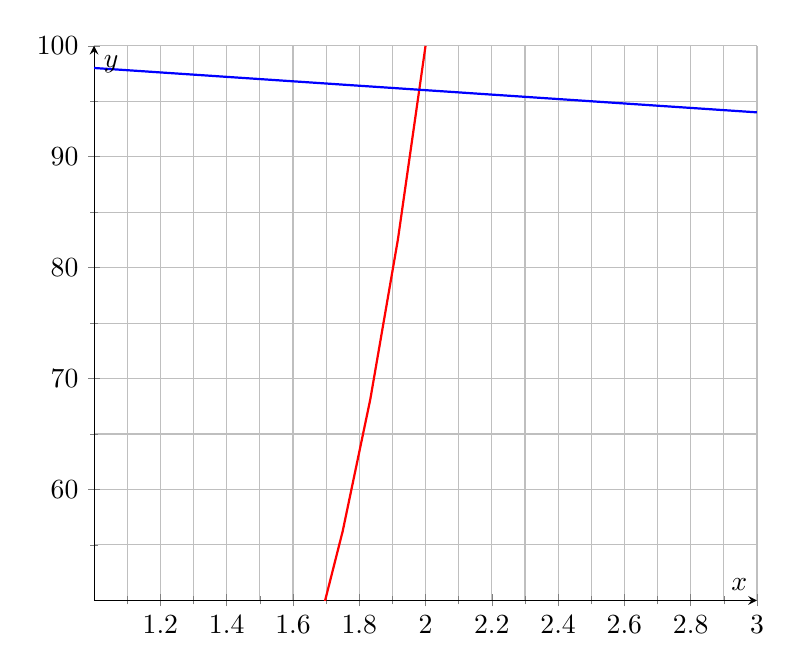
\begin{tikzpicture}
                \begin{axis}[grid=both,ymin=50,ymax=100,xmax=3,xmin=1,
                             minor tick num=1,axis lines = middle,xlabel=$x$,ylabel=$y$]
                    \addplot[red, thick, domain=0:2]{10^x};
                    \addplot[color=blue, thick, domain=0:10]{100-2*x};
                \end{axis}
            \end{tikzpicture}
        \end{center}
        Dengan demikian, akar $x$ dapat dipastikan berada di sekitar $(\num{1,9}; \num{2,0})$.

        \item $\num{-0,874}x^2 + \num{1,75}x + \num{2,627}$ \\
        \penyelesaian $y = \num{-0,874}x^2 + \num{1,75}x + \num{2,627}$, untuk mencari akar-akar persamaan maka $y = 0$. \\

        $\num{-0,874}x^2 + \num{1,75}x + \num{2,627} = 0 \Leftrightarrow \num{0,874}x^2 = \num{1,75}x + \num{2,627}$, diperoleh dua persamaan, $y = \num{0,874}x^2$ dan $y = \num{1,75}x + \num{2,627}$.
        Grafik dari kedua persamaan tersebut diperoleh sebagai berikut.
        \begin{center}
            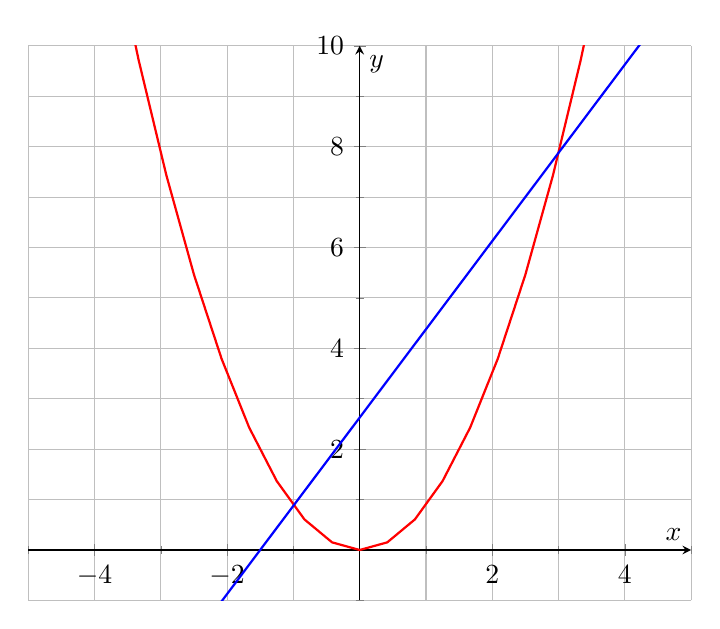
\begin{tikzpicture}
                \begin{axis}[grid=both,ymin=-1,ymax=10,xmax=5,xmin=-5,
                             minor tick num=1,axis lines = middle,xlabel=$x$,ylabel=$y$]
                    \addplot[color=red, thick]{0.874*x^2};
                    \addplot[color=blue, thick]{1.75*x + 2.627};
                \end{axis}
            \end{tikzpicture}
        \end{center}
        Berdasarkan letak perpotongan garis, diperoleh dua akar, yaitu $x_1$ dan $x_2$.\\

        \pagebreak

        Grafik diperbesar pada titik $x_1$:
        \begin{center}
            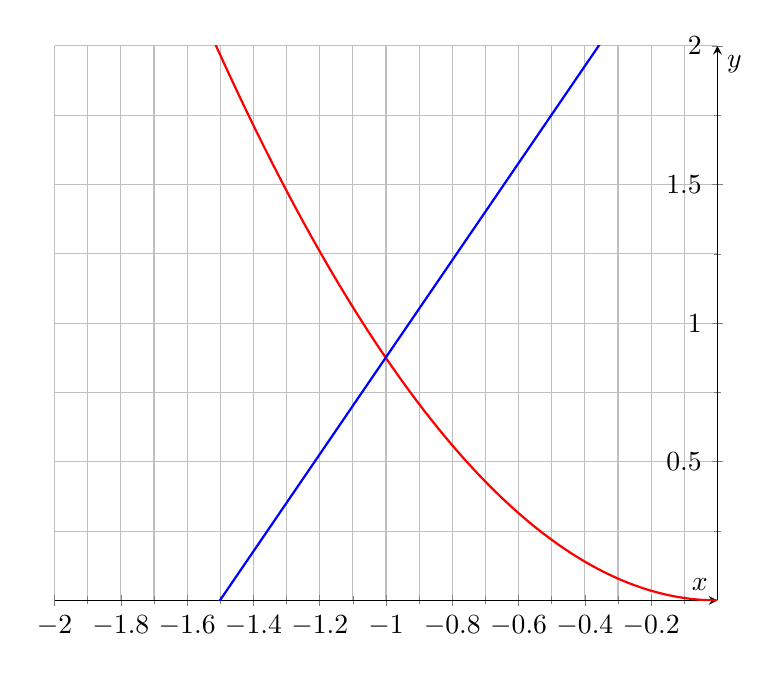
\begin{tikzpicture}
                \begin{axis}[grid=both,ymin=0,ymax=2,xmax=0,xmin=-2,samples=200,
                             minor tick num=1,axis lines = middle,xlabel=$x$,ylabel=$y$]
                    \addplot[color=red, thick, domain=-2:0]{0.874*x^2};
                    \addplot[color=blue, thick, domain=-2:0]{1.75*x + 2.627};
                \end{axis}
            \end{tikzpicture}
        \end{center}

        Grafik diperbesar pada titik $x_2$:
        \begin{center}
            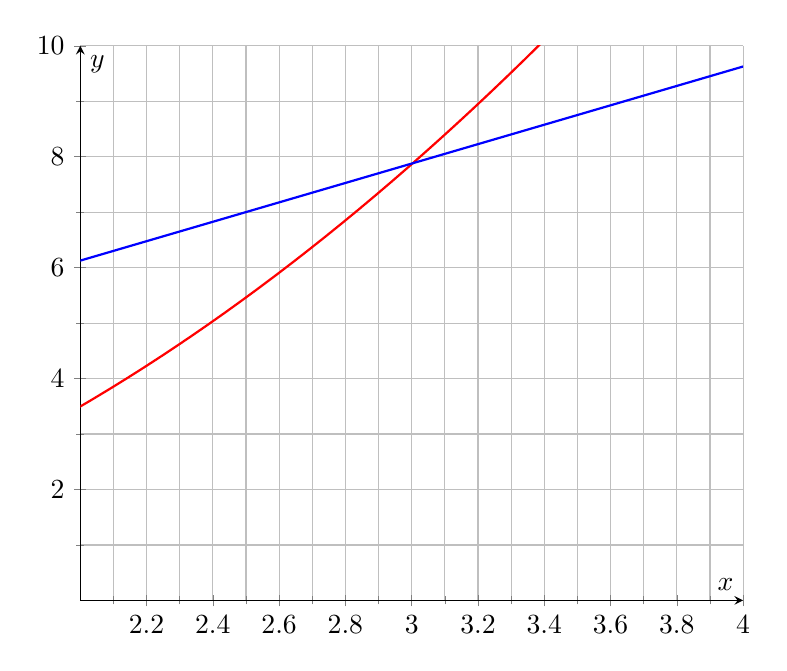
\begin{tikzpicture}
                \begin{axis}[grid=both,ymin=0,ymax=10,xmax=4,xmin=2,samples=200,
                             minor tick num=1,axis lines = middle,xlabel=$x$,ylabel=$y$]
                    \addplot[color=red, thick]{0.874*x^2};
                    \addplot[color=blue, thick]{1.75*x + 2.627};
                \end{axis}
            \end{tikzpicture}
        \end{center}
        Dengan demikian, akar $x_1$ dapat dipastikan terletak di sekitar $(\num{-1,1}; \num{-1,0})$ dan $x_2$ dapat dipastikan terletak di sekitar $(\num{3,0}; \num{3,1})$

        \pagebreak

        \item $\num{-2,1} + \num{6,21}x - \num{3,9}x^2 + \num{0,667}x^3$ \\
        \penyelesaian $y = \num{-2,1} + \num{6,21}x - \num{3,9}x^2 + \num{0,667}x^3$, \\
        $y = 0 \implies \num{-2,1} + \num{6,21}x - \num{3,9}x^2 + \num{0,667}x^3 = 0 \Leftrightarrow \num{2,1} + \num{3,9}x^2 = \num{6,21}x + \num{0,667}x^3$.
        Diperoleh dua persamaan, $y = \num{2,1} + \num{3,9}x^2$ dan $y = \num{6,21}x + \num{0,667}x^3$. \\

        Grafik dari kedua persamaan tersebut diperoleh sebagai berikut.
        \begin{center}
            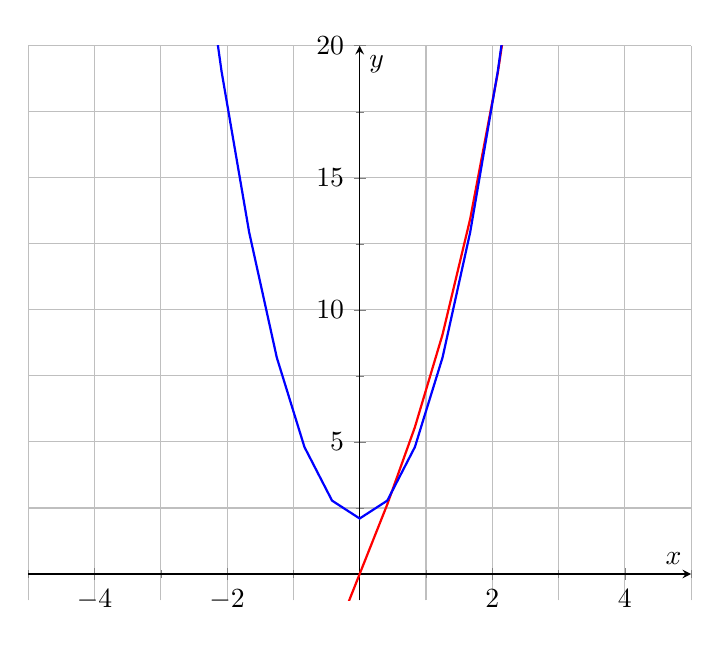
\begin{tikzpicture}
                \begin{axis}[grid=both,ymin=-1,ymax=20,xmax=5,xmin=-5,
                             minor tick num=1,axis lines = middle,xlabel=$x$,ylabel=$y$]
                    \addplot[color=red, thick]{6.21*x + 0.667*x^3};
                    \addplot[color=blue, thick]{2.1 + 3.9*x^2};
                \end{axis}
            \end{tikzpicture}
        \end{center}
        Terlihat bahwa kedua persamaan berpotongan di dua titik berbeda, yaitu $x_1$ dan $x_2$. 
        Kita dapat perbesar grafik di kedua titik tersebut agar dapat melihat informasi yang lebih jelas dari akar-akar persamaannya.\\

        Grafik diperbesar pada titik $x_1$:
        \begin{center}
            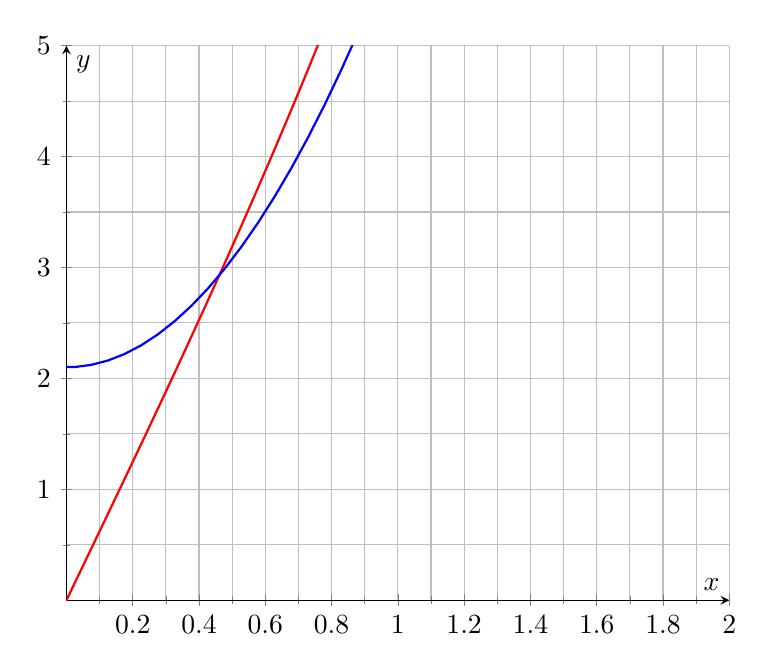
\begin{tikzpicture}
                \begin{axis}[grid=both,ymin=0,ymax=5,xmax=2,xmin=0,samples=200,
                             minor tick num=1,axis lines = middle,xlabel=$x$,ylabel=$y$]
                    \addplot[color=red, thick]{6.21*x + 0.667*x^3};
                    \addplot[color=blue, thick]{2.1 + 3.9*x^2};
                \end{axis}
            \end{tikzpicture}
        \end{center}

        \pagebreak

        Grafik diperbesar pada titik $x_2$:
        \begin{center}
            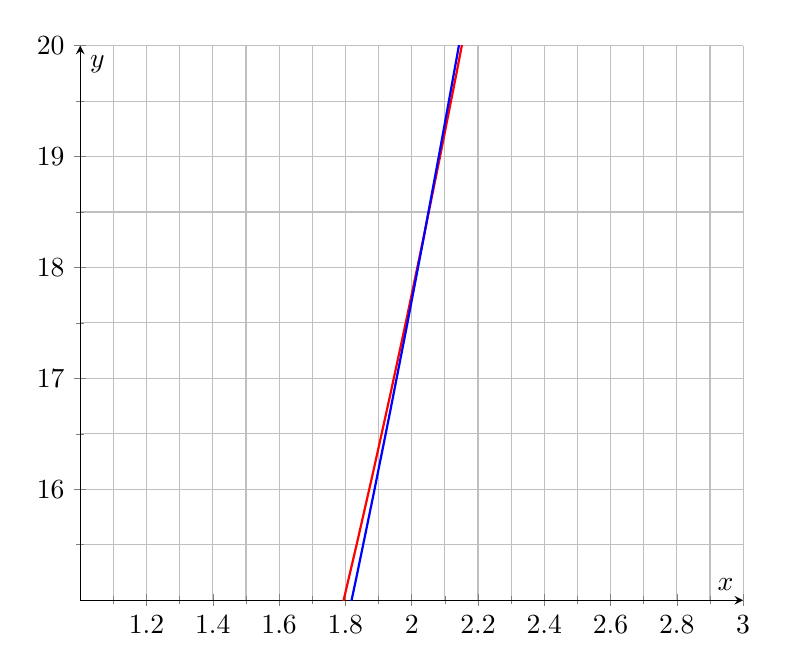
\begin{tikzpicture}
                \begin{axis}[grid=both,ymin=15,ymax=20,xmax=3,xmin=1,samples=200,
                             minor tick num=1,axis lines = middle,xlabel=$x$,ylabel=$y$]
                    \addplot[color=red, thick]{6.21*x + 0.667*x^3};
                    \addplot[color=blue, thick]{2.1 + 3.9*x^2};
                \end{axis}
            \end{tikzpicture}
        \end{center}
        Dengan demikian, dapat dipastikan $x_1$ terletak di sekitar $(\num{0,4}; \num{0,5})$ dan $x_2$ terletak di sekitar $(\num{2,0}; \num{2,1})$.

        \item $(1 - \num{0,6}x)/x$ \\
        \penyelesaian $y = (1 - \num{0,6}x)/x = 1/x - \num{0,6}$, sehingga diperoleh dua persamaan, yaitu $y = 1/x$ dan $y = \num{0,6}$.
        Grafik dari kedua persamaan tersebut diperoleh sebagai berikut.
        \begin{center}
            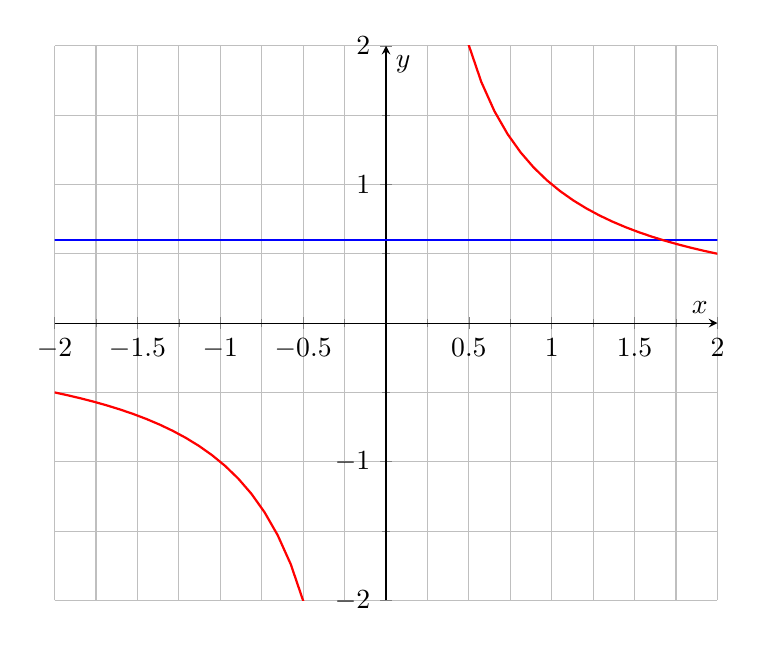
\begin{tikzpicture}
                \begin{axis}[grid=both,ymin=-2,ymax=2,xmax=2,xmin=-2,
                             minor tick num=1,axis lines = middle,xlabel=$x$,ylabel=$y$]
                    \addplot[color=blue, thick]{0.6};
                    \addplot[color=red, thick, domain=-2:-0.1]{1/x};
                    \addplot[color=red, thick, domain=0.1:2]{1/x};
                \end{axis}
            \end{tikzpicture}
        \end{center}
        Berdasarkan letak perpotongan pada grafik, diperoleh informasi bahwa fungsi memiliki satu akar $x$. \\

        \pagebreak
        
        Grafik diperbesar pada akar $x$:
        \begin{center}
            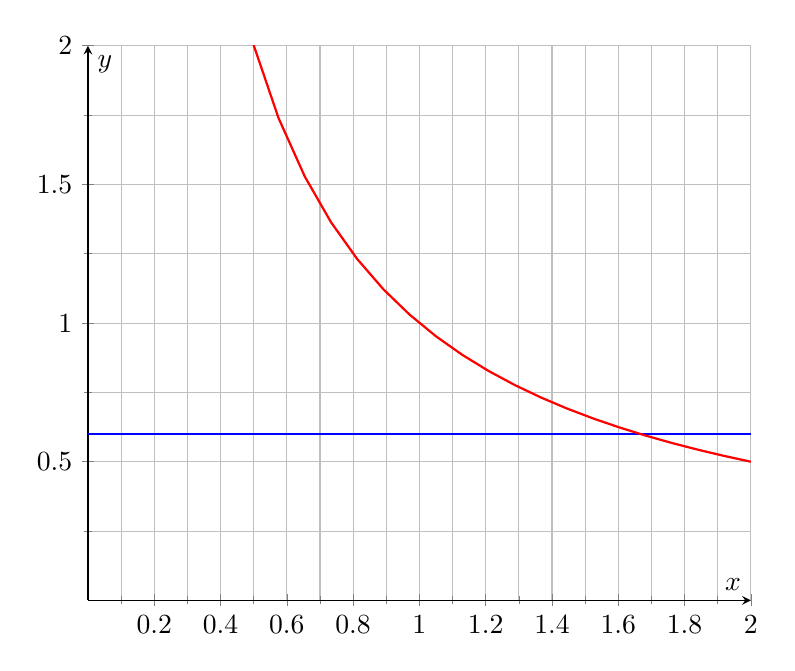
\begin{tikzpicture}
                \begin{axis}[grid=both,ymin=0,ymax=2,xmax=2,xmin=0,
                             minor tick num=1,axis lines = middle,xlabel=$x$,ylabel=$y$]
                    \addplot[color=blue, thick]{0.6};
                    \addplot[color=red, thick, domain=-2:-0.1]{1/x};
                    \addplot[color=red, thick, domain=0.1:2]{1/x};
                \end{axis}
            \end{tikzpicture}
        \end{center}
        Dengan demikian, dapat dipastikan bahwa akar $x$ berada di sekitar $(\num{1,6}; \num{1,7})$. \\
 
    \end{enumerate}
\end{enumerate}

\end{document}